\documentclass[10pt,a4paper]{article}
\usepackage[margin=2.4cm]{geometry}
\usepackage[T1]{fontenc}
\usepackage{lmodern}
\usepackage{microtype}
\usepackage{amsmath,amssymb}
\usepackage{graphicx}
\usepackage{booktabs}
\usepackage{tabularx}
\usepackage{array}
\usepackage{xcolor}
\usepackage{enumitem}
\usepackage[font=small,labelfont=bf]{caption}
\usepackage[authoryear,round]{natbib}
\usepackage[colorlinks=true,linkcolor=blue!50!black,citecolor=blue!50!black,urlcolor=blue!50!black]{hyperref}

\setlength{\parindent}{0pt}
\setlength{\parskip}{0.45em plus 0.1em}
\setlist{nosep,leftmargin=*,topsep=2pt}
\renewcommand{\arraystretch}{1.15}
\renewcommand{\bibfont}{\small}
\setlength{\bibsep}{1.5pt plus 0.5pt}
\newcolumntype{L}{>{\raggedright\arraybackslash}X}

% --- conventions ---------------------------------------------------------------
\newcommand{\code}[1]{\texttt{\detokenize{#1}}}
\newcommand{\exact}{\textcolor{green!45!black}{\textbf{[exact]}}}
\newcommand{\approxt}{\textcolor{orange!85!black}{\textbf{[approx.]}}}
\newcommand{\fitted}{\textcolor{orange!85!black}{\textbf{[fitted]}}}
\newcommand{\measured}{\textcolor{green!45!black}{\textbf{[measured]}}}
\newcommand{\prov}{\textcolor{orange!85!black}{\textbf{[provisional]}}}
\newcommand{\openflag}{\textcolor{red!65!black}{\textbf{[open]}}}
\newcommand{\nbar}{\bar n}
\newcommand{\dtil}{\tilde\delta}
\newcommand{\dhat}{\hat\delta}
\newcommand{\LogU}{\operatorname{LogU}}
\newcommand{\Unif}{\operatorname{U}}
\newcommand{\Pois}{\operatorname{Poisson}}
\newcommand{\E}{\mathbb{E}}
\newcommand{\dd}{\,\mathrm{d}}
\newcommand{\R}{\mathcal{R}}
\newsavebox{\keyboxsave}
\newenvironment{keybox}{\par\smallskip\noindent\begin{lrbox}{\keyboxsave}\begin{minipage}{\dimexpr\linewidth-2\fboxsep-2\fboxrule\relax}\small\setlength{\parskip}{0.4em}}{\end{minipage}\end{lrbox}\fbox{\usebox{\keyboxsave}}\par\smallskip}
\newcommand{\sub}[1]{\par\textit{#1}\ }

\title{\textbf{How the synthetic point patterns are made}\\[3pt]
\large Specification of the DV3 dataset for the AISTATS experiments}
\author{\normalsize point-process-tda, branch \texttt{frontend} at \texttt{559866e}}
\date{\normalsize 14 September 2026}

\begin{document}
\maketitle

\begin{keybox}
\textbf{What this document is.} It specifies every synthetic point pattern the experiments will use: which models, which parameter values, which algorithms, which random numbers, which checks and which jobs. It has three readers. You, to understand the generation process end to end. Your advisors, to audit the design without reading code. An implementer, who should get the same data from it. It contains no code and generated no data. The companion \emph{notes} (\code{docs/theory/notes.pdf}) supply the closed forms; \emph{audit} means \code{docs/status/audit.md}.

\textbf{Tags.} \exact{} the sampler draws from the stated model, up to floating point. \approxt{} an approximation with a stated, checked error. \fitted{} relies on a table fitted to pilot simulations. \measured{} a number measured on data already on disk. \prov{} a number fixed at a review gate after the pilots. \openflag{} unresolved; collected in \S\ref{sec:open}.

\textbf{Where the numbers come from.} \measured{} numbers come from three read-only scripts in \code{docs/theory/scripts/}. \code{inspect_generation.py} reads the existing DV1 clouds and SLURM accounting. \code{design_preview.py} evaluates the closed-form $K$ functions against the saved CSR null tables. \code{make_generation_figures.py} draws the figures. None of them simulates a point pattern. Window $W=[0,1]^2$ throughout.
\end{keybox}

% ============================================================================
\section{The pipeline at a glance}\label{sec:glance}

\begin{figure}[ht]
\centering
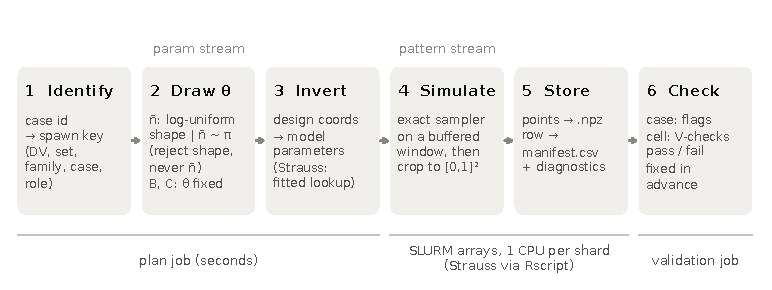
\includegraphics[width=\linewidth]{figs/gen_pipeline.pdf}
\caption{The life of one case. Steps 1--3 are arithmetic, done once for all cases by a planning job. Step 4 is the only simulation. Step 6 aggregates cases into cells and applies the pre-registered checks of \S\ref{sec:valid}. Persistence diagrams and summary curves are computed afterwards by the existing pipeline.}
\label{fig:pipeline}
\end{figure}

Eight sentences summarise the whole design.
\begin{enumerate}
  \item \textbf{Six families.} Poisson (complete spatial randomness, CSR), Thomas, nested Thomas, Mat\'ern hard-core type II, Strauss, and the log-Gaussian Cox process (LGCP).
  \item \textbf{Two kinds of coordinate per parameter vector.} The first is the \emph{expected number of points} $\nbar$. The others are dimensionless \emph{shape} coordinates, with lengths measured in units of the typical point spacing. $\nbar$ is drawn first, log-uniformly on $[100,800]$, identically for every family. The shape is then drawn from the family's prior, rejecting only shapes that violate the family's constraints at that $\nbar$.
  \item \textbf{An inversion turns design coordinates into model parameters.} It is an exact formula for every family except Strauss, which uses a fitted lookup table.
  \item \textbf{Every pattern comes from an exact sampler on a buffered window, cropped to $W$.} Strauss uses dominated coupling from the past (spatstat). LGCP uses circulant embedding plus Poisson cell counts.
  \item \textbf{Four data products} (Table~\ref{tab:products}). A training pool; test set A, drawn i.i.d.\ from the prior; test set B, a grid of fixed parameter cells; test set C, ladders that walk each family down to exact CSR.
  \item \textbf{Every case owns a random stream,} derived from (dataset version, set, family, case, role). Any single case can therefore be regenerated alone.
  \item \textbf{Checks with pass/fail criteria fixed in advance} gate each stage, plus four review gates (D1--D4) at which you look at output before the next stage starts.
  \item \textbf{Cost.} About 1{,}600 CPU-hours of persistence diagrams, the only expensive step. Simulation needs at most 100 CPU-hours, training about 50--80 GPU-hours. The four weeks are limited by people, not compute.
\end{enumerate}

\begin{table}[ht]
\centering\small
\begin{tabularx}{\linewidth}{@{}l l l L L@{}}
\toprule
Set & How drawn & Size & Estimates & Does \emph{not} license\\
\midrule
Training & i.i.d.\ from the prior $\pi$ & $10\,$k per family & (fits the networks; fixed 8{,}500/1{,}500 train/val split) & --\\
A & i.i.d.\ from $\pi$, own seeds & $5\,$k per family & integrated risk under $\pi$; overall accuracy; comparison with other Bayes procedures under the same $\pi$ & regime claims\\
B & fixed $\theta$ per cell, factorial in $(\nbar,\text{scale},\delta)$ & $\approx150$ cells $\times400$ & conditional bias, error and recall at fixed $\theta$ & overall performance; out-of-distribution robustness\\
C & one fixed-shape path per family down to CSR, plus exact Poisson & $54\,$k & detection power and error as functions of $\delta$; the crossover & other paths; overall performance\\
\bottomrule
\end{tabularx}
\caption{The four data products (\S\ref{sec:sets}). About 204{,}000 patterns in total.}
\label{tab:products}
\end{table}

\begin{keybox}
\textbf{What changed since the phase-1 decisions, and why.} The closed-form preview (\code{design_preview.py}) forced four changes.
\begin{enumerate}
\item \emph{The far half of the coverage rule is replaced.} The rule asked for $\ge20\%$ prior mass at $\delta\ge10$. It is unattainable for Mat\'ern~II, whose regularity is physically capped (within its prior interior, $\dtil$ reaches only about 3.5 at $\nbar=125$ and 7 at $500$). At $\nbar=125$ Thomas (9.5\%) and LGCP (2.4\%) could reach it only with distorted priors. Replacement: every B cell up to $\dtil=8$ that the family can reach must lie in the interior of its prior. The near-CSR half ($\ge20\%$ at $\delta\le1$) is kept. It is met by every closed-form family at every B-level $\nbar$ (25--53\%); Strauss is checked at D1.
\item \emph{Thomas $\mu_{\min}$ moves from 0.2 to 0.1.} This lifts the near-CSR mass at $\nbar=500$ from 17.6\% to 26.9\%.
\item \emph{Nested $\mu_2$ now goes down to 0.03.} Without this the nested ladder cannot get below $\dtil\approx1.1$.
\item \emph{Mat\'ern~II's B and C levels are set in $\tau$, not $\delta$.} $\delta_L$ jumps when the hard-core radius crosses the $r=0.01$ floor of the $L$ statistic (\S\ref{sec:delta}).
\end{enumerate}
\end{keybox}

% ============================================================================
\section{Design philosophy}\label{sec:philosophy}

\textbf{What the data must support.} The paper makes three kinds of claim, and each needs its own data.
\begin{itemize}
  \item[(C1)] \emph{Overall.} ``Averaged over the prior $\pi$, method $X$ has risk $R_X$.'' This needs an i.i.d.\ sample from $\pi$ (set A). The number means something only relative to $\pi$, and it is directly comparable with any Bayes procedure that uses the same $\pi$, such as ABC random forests \citep{Raynal2019}.
  \item[(C2)] \emph{Regime.} ``At parameter values whose departure from CSR is $\delta$, with $\nbar$ expected points, method $X$ has conditional error $e_X(\delta,\nbar)$.'' This needs fixed parameter values with replication (set B).
  \item[(C3)] \emph{Boundary.} ``As a pattern approaches CSR along a fixed-shape path, method $X$ keeps detecting structure down to $\delta\approx\delta^\ast$.'' This needs dense one-dimensional paths that end at exact CSR (set C). It is the headline figure.
\end{itemize}

\textbf{Why the current (DV1) data cannot support C2 or C3} (Fig.~\ref{fig:delta}a).
\begin{itemize}
  \item No clustered DV1 cloud is statistically close to CSR: 0 of 7{,}000 Thomas clouds have $S_L\le1$ \measured.
  \item Difficulty is tied to sample size: Spearman$(n,S_L)=0.62$ for Thomas and $0.69$ for nested \measured. A regime effect and a sample-size effect cannot be told apart.
  \item Strauss is the reverse: 28\% of its clouds are near CSR (notes, departure-measure subsection), but its parameters were drawn in raw coordinates, so its regimes were never controlled.
\end{itemize}

\textbf{Five principles.} Each principle is followed by what it buys.
\begin{enumerate}
  \item[P1] \emph{Separate ``how many points'' from ``what structure''.} $\nbar$ is drawn first, from the same distribution for every family, and no structure parameter changes it. Think of $\nbar$ as the size of the sample and the shape as the picture: you can change one without changing the other. \emph{Buys:} sample size becomes a factor you control; $n(x)$ stops leaking the class in classification.
  \item[P2] \emph{Measure structure in units of the point spacing} $\ell=\nbar^{-1/2}$. A cluster with standard deviation $\sigma$ has scale $s=\sigma/\ell=\sigma\sqrt{\nbar}$. \emph{Buys:} at fixed shape, changing $\nbar$ changes only the noise level (Fig.~\ref{fig:delta}b). DTM-$k$ features, which are tied to the spacing through $k$, see the same geometry at every $\nbar$.
  \item[P3] \emph{Reach CSR from inside the prior.} Every family keeps at least 20\% of its prior mass within $\delta\le1$ at every B-level $\nbar$. \emph{Buys:} near-CSR evaluation is interpolation, not extrapolation.
  \item[P4] \emph{Exact where possible; a stated, checked error elsewhere.} Every sampler is exact for its model on a buffered window (for Strauss, wherever coupling from the past is feasible). The remaining approximations are edge truncation, the LGCP grid and the Strauss lookup. Each has an error bound and a pass/fail check. \emph{Buys:} no referee argument about burn-in or simulation error.
  \item[P5] \emph{Every case is reproducible alone.} It has its own random stream, and it is stored with its seed and sampler diagnostics. \emph{Buys:} any suspicious pattern can be regenerated and inspected in isolation.
\end{enumerate}

\textbf{The prior is a design choice, and the paper says so.} Log-uniform laws in dimensionless coordinates are the conventional ``scale-free'' choice. They are not a claim about nature. Because $\pi$ is known exactly, A can be reweighted to any other prior with the same support using importance weights, at no cost. Report that sensitivity for the headline A numbers.

% ============================================================================
\section{Coordinates: how a pattern's regime is described}\label{sec:coords}

\subsection{Window, spacing and $\nbar$}
With $|W|=1$ the intensity equals the expected count, $\lambda=\nbar$. The \emph{spacing} is $\ell=\nbar^{-1/2}$: under CSR the mean nearest-neighbour distance is $\ell/2$. Every length parameter is reported both in window units and in spacings (e.g.\ $s=\sigma\sqrt{\nbar}$). $\nbar$ lives in parameter space. The realised count $n(x)$ scatters around it: overdispersed for clustered families, underdispersed for regular ones.

\subsection{$\delta$: distance from CSR as the classical test sees it}\label{sec:delta}
\textbf{Intuition.} Compute the $L$-function of a pattern. Under CSR, $\hat L(r)-r$ wiggles around its null mean. Ask how many null standard deviations the model's \emph{expected} curve stands away from that mean at its worst radius, then divide by the 5\% critical value. So $\delta\approx1$ means the typical pattern sits at the edge of detectability. $\delta\gg1$ means structure is obvious, and $\delta\ll1$ means the model is indistinguishable from CSR by this test.

\textbf{Definition.} Let $\hat\Phi_x(r)=\hat L_x(r)-r$ be computed with the repo's estimator: Ripley isotropic edge correction, $\hat\lambda^2=n(n-1)$, 513 radii on $[0,0.25]$. The null tables come from binomial patterns with $n$ points. They give the mean $m_0(r;n)$ and s.d.\ $s_0(r;n)$ of $\hat\Phi$, and the 95\% quantile $c_{0.95}(n)$ of $\max_r|\hat\Phi-m_0|/s_0$ on held-out null replicates. The radius range is $\R=[0.01,0.25]$. Then
\begin{equation}
\delta(\theta,\nbar)=\frac{1}{c_{0.95}(\nbar)}\,\max_{r\in\R}\frac{\big|\E_\theta\hat\Phi(r)-m_0(r;\nbar)\big|}{s_0(r;\nbar)}.
\label{eq:delta}
\end{equation}
Studentising each radius follows the global envelope tests of \citet{Myllymaki2017}. $\delta$ is a parameter-space quantity. It depends on the model and $\nbar$, and also on the window, the estimator and $\R$: it measures difficulty \emph{for this test}. It is computed in two ways.
\begin{itemize}
  \item $\dtil$ (design time): replace $\E_\theta\hat\Phi$ by the closed-form $L_\theta(r)-r$. This places the B cells and the C levels. Strauss has no closed form, so it uses pilot tables (\S\ref{sec:strauss}).
  \item $\dhat$ (analysis time): the mean curve over a cell's replicates, which includes the estimator's own bias. Every reported result uses $\dhat$. Averaging 400 curves adds an upward bias of about $0.05$ in $\delta$, which is negligible.
\end{itemize}

\textbf{Why $\delta$ grows like $\sqrt{\nbar}$} (derivation in App.~\ref{app:counting}). Near CSR, $\hat K(r)$ counts pairs, and pair counts are nearly Poisson, so $\operatorname{sd}\hat K(r)\approx\sqrt{2\pi}\,r/\nbar$. A process with $K=\pi r^2+e(r)$ therefore stands $z(r)\approx\nbar\,e(r)/(\sqrt{2\pi}\,r)$ standard deviations from CSR. For Thomas this gives the rule of thumb $\delta\approx0.04\,\mu\sqrt{\nbar}/s$. It reproduces the exact $\dtil$ of Fig.~\ref{fig:delta}b to within about 20\%.

\textbf{Secondary coordinates.} $\delta_G$ and $\delta_F$ apply (\ref{eq:delta}) to the nearest-neighbour and empty-space functions, on the radii where their null s.d.\ exceeds 10\% of its maximum, as in the notes.

\textbf{A blind spot the preview exposed.} $\R$ starts at $r=0.01$ in window units. Structure at smaller scales is invisible to $\delta_L$, even when $G$ detects it easily. For Mat\'ern~II at $\nbar=250$ that means any hard-core radius below $0.01$, i.e.\ $\tau<0.16$. The pattern then has a visible nearest-neighbour gap but $\dtil_L\le1$, and $\dtil_L$ jumps as $R$ crosses $0.01$ (Fig.~\ref{fig:ladders}, last panel). So inhibitory families report $\delta_G$ alongside $\delta_L$, and Mat\'ern~II's test sets are laid out in $\tau$. Whether $\delta_G$ should become primary for inhibitory families is decided at D1 \openflag.

\begin{figure}[t]
\centering
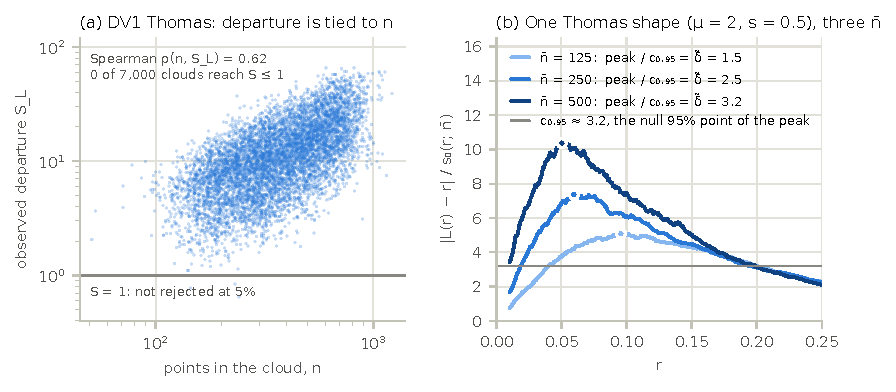
\includegraphics[width=\linewidth]{figs/gen_delta.pdf}
\caption{(a) Existing DV1 Thomas data: departure $S_L$ against the point count. No cloud is near CSR, and departure rises with $n$. (b) What $\delta$ measures. The studentised distance $|L(r)-r|/s_0(r;\nbar)$ of one Thomas shape at three $\nbar$. $\dtil$ is the peak divided by $c_{0.95}$. The shape is fixed, so only the noise level changes, and $\dtil$ grows roughly as $\sqrt{\nbar}$. The jaggedness is Monte Carlo noise in the 200-replicate null s.d.; WP2 rebuilds the null tables with 2{,}000 replicates.}
\label{fig:delta}
\end{figure}

\subsection{$S$: the test-time twin of $\delta$}\label{sec:S}
The label-free departure measure of the notes (``A label-free departure measure'') is $S(x)$: formula (\ref{eq:delta}) with the realised curve $\hat\Phi_x$ and the realised $n(x)$ in place of the expectation and $\nbar$. It is not the same object as $\delta$. The two are related as follows (Fig.~\ref{fig:svd}):
\begin{itemize}
  \item At $\delta=0$, $S$ follows its null law: $P(S\le1)=0.95$ by construction, and the median is 0.58--0.65 for $n=100$--$800$ \measured.
  \item At matched $n$, $\E[S\mid\theta]\ge\delta$, by Jensen's inequality (a supremum of absolute values is convex), and $S/\delta\to1$ as $\delta$ grows. $S$ is biased upward near CSR.
  \item Along a fixed-shape ladder (\S\ref{sec:ladders}) the expected curve scales with the amplitude $a$, and $\E\sup_r|a\,h(r)+\varepsilon(r)|$ is convex and even in $a$. So $\E[S]$ rises with $a$, and hence with $\delta$: the two are monotonically related \emph{in expectation}. This is exact if the noise $\varepsilon$ does not change along the ladder, and approximate otherwise (clustering inflates it).
  \item Across families, the same $\delta$ does not give the same law for $S$. A deviation spread over many radii and one concentrated at a single radius produce different noisy maxima.
\end{itemize}
\textbf{Consequence for the regime-gated hybrid.} The gate sees only $S$. So it learns $B(S)=\int A(\delta)\,p(\delta\mid S)\dd\delta$, a version of the expert-advantage curve $A(\delta)$ blurred by $p(\delta\mid S)$, which is wide near CSR. A crossover located in $\delta$ with set C will appear flattened and shifted in $S$. Report the headroom as a chain: per-cloud oracle $\ge$ gate on the true $\delta$ $\ge$ gate on $S$. Bin evaluations by $\dhat$, never by $S$: binning by $S$ selects on the classical expert's own noise.

\begin{figure}[t]
\centering
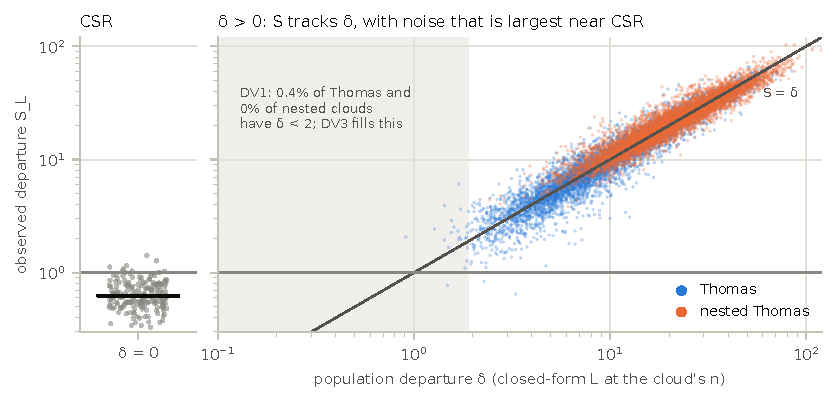
\includegraphics[width=\linewidth]{figs/gen_s_vs_delta.pdf}
\caption{Observed $S_L$ against the population departure for the DV1 test clouds (closed-form $L$ at each cloud's $n$), with the null law of $S$ at $\delta=0$ on the left ($n=400$). $S$ tracks $\delta$ at large $\delta$ and is noisy near it. In DV1, 0.4\% of Thomas and none of the nested clouds lie below $\delta=2$. That empty band is what DV3 fills.}
\label{fig:svd}
\end{figure}

\subsection{$\tau$ and direction}
$\tau=\sqrt{\nbar}\,r_{1/2}(\theta)$, where $r_{1/2}$ is the radius at which $|K(r)-\pi r^2|$ reaches half its limit as $r\to\infty$. It is the scale of the structure in spacings, and a parameter-space quantity.
\begin{itemize}
  \item Thomas: $\tau=2\sqrt{\ln2}\,s=1.665\,s$.
  \item LGCP: $r_{1/2}/s=1.67,\,1.53,\,1.16$ at $\sigma^2=0.1,1,3$ \measured.
  \item Mat\'ern~II: $r_{1/2}/R=0.71$--$0.65$ for $\tau=0.1$--$0.5$ \measured.
  \item Nested: two values, one per step of $K$.
  \item Strauss: from the pilot tables.
\end{itemize}
$\tau$ is an analysis covariate. B is laid out in each family's own scale coordinate. The \emph{direction} is the sign of $K-\pi r^2$ at $r_{1/2}$: positive (clustered) for Thomas, nested and LGCP, negative (regular) for Mat\'ern~II and Strauss. It is fixed by family, so here it is a label, not a design factor.

\subsection{Paths to CSR (degeneration ladders)}\label{sec:ladders}
Most families approach CSR in more than one way. For example, Thomas becomes CSR as clusters get small ($\mu\to0$) or diffuse ($s\to\infty$). Set C uses one \emph{canonical ladder} per family: the path along which the excess pair correlation $g-1$ shrinks towards zero \emph{with its shape fixed}, holding $\nbar$ and the scale fixed. At the same $\delta$, families on these ladders then differ only in the shape of their departure (Table~\ref{tab:ladders}, Fig.~\ref{fig:ladders}).

\begin{table}[ht]
\centering\small
\begin{tabularx}{\linewidth}{@{}l L l L l l@{}}
\toprule
Family & CSR limits & Canonical ladder & Is the shape fixed? & \multicolumn{2}{c}{$\dtil$ range in C \measured}\\
\cmidrule(l){5-6}
 & & & & low $\nbar$ & high $\nbar$\\
\midrule
Thomas & $\mu\to0$; $s\to\infty$ & $\mu\downarrow$ at $s=1$ & exactly: $K-\pi r^2=\frac{\mu}{\nbar}(1-e^{-r^2/4\sigma^2})$ & 0.10--5.4 & 0.15--10\\
Nested & both levels must dissolve & $\mu_2\downarrow$ at $\mu_1=3,\rho=6,s_2=0.2$ & exactly: both step masses $\propto\mu_2$ & 0.22--10 & 0.27--10\\
Mat\'ern II & $\tau\to0$ & $\tau\downarrow$ & no: one parameter moves range and amplitude together & 0.14--3.5 & 0.15--7.1\\
Strauss & $\gamma\to1$; $\tau\to0$ & $\gamma\uparrow1$ at $\tau=0.5$ & to first order in $1-\gamma$ & \prov & \prov\\
LGCP & $\sigma^2\to0$; $s\sqrt{\nbar}\to0$ & $\sigma^2\downarrow$ at $s\sqrt{\nbar}=1$ & to first order: $g-1=\sigma^2e^{-r/s}+O(\sigma^4)$ & 0.18--6.2 & 0.39--10\\
\bottomrule
\end{tabularx}
\caption{Canonical ladders. The $\dtil$ range is spanned by the amplitude parameter's interior range (central 80\% of its prior), clipped to $[0.1,10]$. Low/high $\nbar$ is 125/500, or 250/500 for nested.}
\label{tab:ladders}
\end{table}

\begin{figure}[t]
\centering
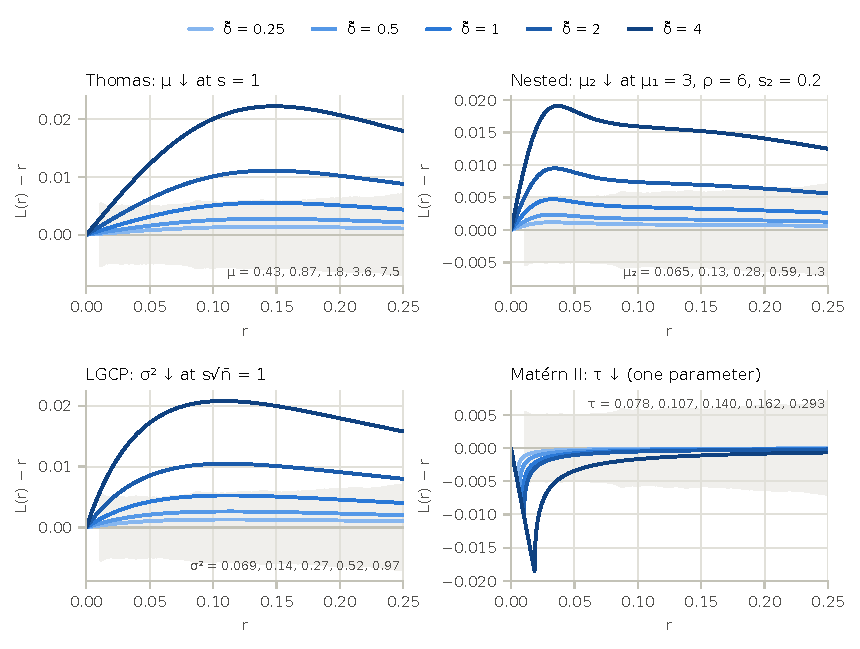
\includegraphics[width=\linewidth]{figs/gen_ladders.pdf}
\caption{The ladders at $\nbar=250$: closed-form $L(r)-r$ at five values of $\dtil$. The same colour means the same $\dtil$ in every panel. The grey band is $\pm c_{0.95}\,s_0(r)$: a curve that stays inside it at every radius has $\dtil\le1$. The first three ladders scale one fixed shape. Mat\'ern~II cannot. Its deficit lives below $r\approx R$, and $\dtil$ jumps when $R$ crosses the $r=0.01$ floor (from $\tau=0.140$ to $0.162$ between $\dtil=1$ and $2$). Strauss has no closed form.}
\label{fig:ladders}
\end{figure}

% ============================================================================
\section{The six families}\label{sec:families}

Each family follows the same layout: intuition, model, design coordinates and inversion, sampler and why it is correct, prior and why, path to CSR, and what can go wrong. All priors are summarised in Table~\ref{tab:prior}.

\subsection{Poisson (CSR)}
\sub{In one sentence.} Points are dropped independently and uniformly; there is no interaction at any scale.
\sub{Sampler} \exact. Draw $N\sim\Pois(\nbar)$, then $N$ i.i.d.\ uniform points in $W$.
\sub{Prior.} $\nbar\sim\LogU[100,800]$ only.
\sub{Role.} A class in classification. The $\delta=0$ anchor of C. Its binomial variant ($N$ fixed at $n$) builds the null tables for $\delta$ and $S$. Do not mix the two: $S$ conditions on $n(x)$, so its null is binomial.

\subsection{Thomas}
\sub{In one sentence.} Invisible parents scatter a random number of children around themselves with a Gaussian spread, and only the children are observed \citep{Thomas1949,NeymanScott1958}.
\sub{Model.} Parents form a Poisson process of intensity $\kappa$. Each parent has $\Pois(\mu)$ children, displaced by $N(0,\sigma^2I)$. So $\lambda=\kappa\mu$, and $K(r)=\pi r^2+(1-e^{-r^2/4\sigma^2})/\kappa$ (notes, eq.~1). $\mu$ is both the mean cluster size and the expected number of ``extra'' neighbours of a typical point.
\sub{Design coordinates and inversion} \exact. $(\nbar,\mu,s)$ with $s=\sigma\sqrt{\nbar}$, the cluster s.d.\ in spacings. The inversion is $\kappa=\nbar/\mu$, $\sigma=s/\sqrt{\nbar}$. $\E n=\kappa\mu|W|=\nbar$ holds exactly, because of the buffer.
\sub{Sampler} \exact{} up to a truncation below $10^{-5}$.
\begin{enumerate}
  \item Set the buffer to $b=\sigma\,\Phi^{-1}(1-10^{-4})=3.719\,\sigma$.
  \item Draw $N_p\sim\Pois(\kappa(1+2b)^2)$ parents, uniform on $[-b,1+b]^2$.
  \item Give each parent $\Pois(\mu)$ children with $N(0,\sigma^2I)$ offsets.
  \item Keep the children that fall in $W$.
\end{enumerate}
\emph{Why correct:} this is the definition of the process restricted to $W$. The only error is from parents beyond the buffer. They miss at most a fraction $4\sigma\,\E(Z-3.719)^+\approx10^{-4}\sigma<10^{-5}$ of the expected points (App.~\ref{app:buffer}). Repo: \code{neyman_scott.py}, reused unchanged. It takes milliseconds even at $\mu=0.1$, where $\kappa$ reaches 8{,}000.
\sub{Prior.} $\mu\sim\LogU[0.1,30]$ and $s\sim\LogU[0.1,1.5]$, with two constraints: $\sigma\le0.1$ and $\kappa\ge5$.
\begin{itemize}
  \item $\mu=0.1$ gives patterns that are CSR plus a few sibling pairs, which reaches CSR from inside.
  \item $\mu\le30$ allows clusters of up to 30 points, while $\kappa\ge5$ keeps at least five clusters in $W$. At $\nbar=125$ this caps $\mu$ at 25.
  \item $s<0.1$ adds nothing: the children are already on top of each other.
  \item $s>1.5$ gives clusters wider than 1.5 spacings, which overlap heavily and run into $\sigma\le0.1$ (a cluster s.d.\ of at most a tenth of the window).
\end{itemize}
The constraints reject 14\% of shape draws at $\nbar=125$ and none at $\nbar\ge250$ \measured. Near-CSR mass ($\dtil\le1$) is 40\%, 32\% and 27\% at $\nbar=125,250,500$ \measured.
\sub{Path to CSR.} $\mu\downarrow$ at $s=1$. The excess $K$ is exactly proportional to $\mu$ (Table~\ref{tab:ladders}).
\sub{What can go wrong.}
\begin{itemize}
  \item At small $\mu$, $\sigma$ is not identified: only the product $\mu/\nbar$ times a shape appears. Estimates regress to the prior. This is expected and reported as skill.
  \item With few clusters ($\kappa$ small), $\hat K$ is noisy. The constraint $\kappa\ge5$ limits this.
  \item DV1 paired every Thomas cloud with a Mat\'ern-cluster ``twin'' (audit \S5.14). Both causes are gone: the family is part of the seed, and Mat\'ern cluster is dropped.
\end{itemize}

\subsection{Nested Thomas}\label{sec:nested}
\sub{In one sentence.} Clusters of clusters: meta-parents scatter parents, parents scatter children.
\sub{Model.}
\begin{itemize}
  \item Meta-parents form a Poisson process of intensity $\kappa$.
  \item Each meta-parent has $\Pois(\mu_1)$ parents, displaced by $N(0,\sigma_1^2I)$.
  \item Each parent has $\Pois(\mu_2)$ children, displaced by $N(0,\sigma_2^2I)$.
\end{itemize}
So $\lambda=\kappa\mu_1\mu_2$. $K$ has two steps (notes, eq.~2). The inner step, at $r\approx2\sigma_2$, has mass $\mu_2/\nbar$; the outer step, at $r\approx2(\sigma_1^2+\sigma_2^2)^{1/2}$, has mass $\mu_1\mu_2/\nbar$.
\sub{Design coordinates and inversion} \exact. $(\nbar,\mu_1,\mu_2,s_2,\rho)$ with $s_2=\sigma_2\sqrt{\nbar}$ and $\rho=\sigma_1/\sigma_2$. The inversion is $\kappa=\nbar/(\mu_1\mu_2)$, $\sigma_2=s_2/\sqrt{\nbar}$, $\sigma_1=\rho\,\sigma_2$.
\sub{Sampler} \exact{} up to two truncations below $10^{-5}$ each. There is no library sampler, but the construction is standard. The meta-level is itself a Thomas process, simulated on $W\oplus b_2$ with its own buffer $b_1=3.719\,\sigma_1$. Its points are the parents, whose children use $b_2=3.719\,\sigma_2$. Repo: \code{nested_thomas.py}, reused unchanged. The notes verified its $K$ against simulation (notes, Fig.~2).
\sub{Prior.} $\mu_1\sim\LogU[1.5,6]$, $\mu_2\sim\LogU[0.03,20]$, $s_2\sim\LogU[0.05,0.5]$, $\rho\sim\LogU[3,12]$, with constraints $\kappa\ge15$ and $2(\sigma_1^2+\sigma_2^2)^{1/2}\le0.2$.
\begin{itemize}
  \item $\mu_1\ge1.5$: otherwise most meta-parents have fewer than two parents and there is no second level.
  \item $\rho\ge3$ keeps the two steps of $K$ apart.
  \item The outer-scale constraint keeps meta-clusters within a fifth of the window.
  \item $\kappa\ge15$ is the identifiability constraint. $\mu_1$ is identified only through the ratio of outer to inner step mass, whose precision scales like $1/\sqrt{\kappa}$. In DV1, with $\kappa\in[15,120]$, every method (curves or topology) had MSE $\approx0.45$ on the z-scored $\log\mu_1$, i.e.\ about 30\% error \measured.
\end{itemize}
The constraints bind hard at small $\nbar$: acceptance is 39\%, 56\% and 76\% at $\nbar=125,250,500$ \measured. The nested shape prior therefore really does depend on $\nbar$, which is why nested B and C use $\nbar\in\{250,500\}$ only. Near-CSR mass is 44\%, 32\% and 26\%.
\sub{Path to CSR.} $\mu_2\downarrow$ at $\mu_1=3$, $\rho=6$, $s_2=0.2$. Both step masses are proportional to $\mu_2$.
\sub{What can go wrong.}
\begin{itemize}
  \item $\mu_1$ is weakly identified; report it separately and never average it into a headline.
  \item At $\mu_2<1$ most parents leave at most one child, so the inner level fades from view first.
  \item Near $\rho=3$ with similar step masses, the steps merge.
\end{itemize}

\subsection{Mat\'ern hard-core type II}\label{sec:m2}
\sub{In one sentence.} Throw candidate points with random ``ages'', then delete every candidate that has an older one within distance $R$; the survivors are at least $R$ apart \citep{Matern1986}.
\sub{Model.} Primary points form a Poisson process of intensity $\lambda_p$, with i.i.d.\ $\Unif(0,1)$ marks. A point is deleted if some other primary point within $R$ has a smaller mark. The intensity is $\lambda=(1-e^{-\lambda_p\pi R^2})/(\pi R^2)$, and $g$ is in closed form (notes, eq.~3).
\sub{Design coordinates and inversion} \exact. $(\nbar,\tau)$ with $\tau=R\sqrt{\nbar}$. The inversion is $R=\tau/\sqrt{\nbar}$ and $\lambda_p=\nbar\,[-\ln(1-\pi\tau^2)]/(\pi\tau^2)$ (App.~\ref{app:m2}). It needs $\pi\tau^2<1$, i.e.\ $\tau<0.564$.
\sub{Sampler} \exact.
\begin{enumerate}
  \item Draw the primary process on $W\oplus R$.
  \item Thin it.
  \item Crop to $W$.
\end{enumerate}
\emph{Why correct:} whether $x\in W$ survives depends only on primaries in the disc $b(x,R)\subset W\oplus R$, and all of those are simulated. \emph{Repo bug to fix in WP1:} \code{matern.py:34-52} thins inside $W$ only. Candidates just outside $W$ never delete edge points, so the edge band ends up with 1.149 times the interior intensity (notes, Mat\'ern~II subsection).
\sub{Prior.} $\tau\sim\LogU[0.05,0.55]$.
\begin{itemize}
  \item At $\tau=0.55$ we have $\pi\tau^2=0.95$ and about $3.2\,\nbar$ candidates, near saturation.
  \item At $\tau=0.05$, only 0.8\% of CSR points would have a neighbour within $R$.
\end{itemize}
Near-CSR mass is 40--45\%. $\dtil\ge10$ is impossible for this family \measured.
\sub{Path to CSR.} $\tau\downarrow$, with no fixed-shape option (Table~\ref{tab:ladders}). B and C use log-spaced $\tau$ levels (\S\ref{sec:sets}).
\sub{What can go wrong.}
\begin{itemize}
  \item Only weak regularity is possible (packing fraction $\le1/4$).
  \item The $\delta_L$ blind spot below $r=0.01$ (\S\ref{sec:delta}).
  \item The edge bug, if the fix is missed. Check V4 catches it.
\end{itemize}

\subsection{Strauss}\label{sec:strauss}
\sub{In one sentence.} A Gibbs model in which every pair of points closer than $R$ costs a factor $\gamma\in[0,1]$: $\gamma=1$ is Poisson, $\gamma=0$ is a hard core \citep{Strauss1975,KellyRipley1976}.
\sub{Model.} The density with respect to a unit-rate Poisson process on the simulation window is $f(x)\propto\beta^{n(x)}\gamma^{s_R(x)}$, where $s_R(x)$ counts the $R$-close pairs. $\beta$ is an \emph{activity}, not an intensity: $\lambda<\beta$, with no closed form.
\sub{Design coordinates and inversion} \fitted. The design coordinates are $(\nbar,\tau,\gamma)$ with $\tau=R\sqrt{\nbar}$. Scale invariance does the heavy lifting (App.~\ref{app:scale}). If $X$ is Strauss$(\beta,\gamma,R)$, then the rescaled pattern $aX$ is Strauss$(\beta/a^2,\gamma,aR)$. So $\lambda R^2=h(\beta R^2,\gamma)$ is a function of two arguments, not three. The inversion is therefore a two-dimensional table:
\begin{enumerate}
  \item In WP2, estimate $h$ by pilot simulation on a grid over $(\log\beta R^2,\gamma)$.
  \item For each $\gamma$, invert $h$ in $\beta R^2$ by monotone interpolation.
  \item Set $R=\tau/\sqrt{\nbar}$ and $\beta=h^{-1}(\tau^2,\gamma)/R^2$.
\end{enumerate}
The table's starting guess is the Poisson-saddlepoint approximation of \citet{BaddeleyNair2012}. Its form $\lambda=W_0(\beta G)/G$ with $G=(1-\gamma)\pi R^2$ is confirmed by \citet{CoeurjollyLavancier2018}. It inverts to $\beta R^2=\tau^2e^{(1-\gamma)\pi\tau^2}$.

Evidence that the table is enough comes from the 8{,}000 DV1 Strauss clouds \measured:
\begin{itemize}
  \item A two-dimensional fit of $\log n R^2$ leaves residual s.d.\ $0.053$. That is pure sampling noise: Poisson scale is $0.059$, and Strauss counts are underdispersed.
  \item Adding $\log R$ as a third covariate changes the residual in the fifth decimal, so finite-window effects are negligible.
  \item The saddlepoint approximation itself is off by $-18\%$ to $+11\%$.
\end{itemize}
\emph{Worked example.} Take $\nbar=250$, $\tau=0.5$, $\gamma=0.3$, so $R=0.0316$. The saddlepoint approximation gives $\beta=433$; the DV1 lookup gives $475$ (10\% higher). \emph{Check:} in every B and C cell, mean $n$ must match $\nbar$ within $\max(3\text{ s.e.},1\%)$ (V0).
\sub{Sampler} \exact{} on $W\oplus2R$. We use dominated coupling from the past, as implemented by \code{spatstat.random::rStrauss} (version 3.5-1; \citealp{Baddeley2015}) \citep{ProppWilson1996,KendallMoller2000,BerthelsenMoller2002,BerthelsenMoller2003}.

\begin{keybox}
\textbf{Why coupling from the past gives an exact draw.} A Markov chain started at time $-T$ and run to time $0$ gives an exact draw if its state at $0$ no longer depends on where it started. Coupling from the past makes that checkable: run coupled copies of the chain from \emph{every} possible starting state with the same random numbers. If they have all merged by time $0$, the common state is what a chain started infinitely long ago would show, i.e.\ an exact draw.

For point processes, ``every starting state'' is handled by a \emph{dominating process}. This is a free birth--death process with birth rate $\beta$ and unit death rate, whose stationary law is Poisson$(\beta)$. It is reversible, so it is easy to run backwards in time. Every Strauss chain can be obtained by thinning it, so an \emph{upper} and a \emph{lower} chain sandwich all Strauss chains. If upper and lower meet by time $0$, output their common state. If not, start twice as far in the past, reusing the randomness already drawn. The output is exact whenever the algorithm finishes; there is no burn-in to choose.
\end{keybox}

\begin{itemize}
  \item \emph{Boundary.} \code{rStrauss} simulates on $W$ expanded by $2R$ (\code{expandwinPerfect(W, expand, rmhexpand(distance=2*R))}) and crops. The draw is exact for the free-boundary Strauss process on $W\oplus2R$, and approximate for the stationary process on $W$. This is the same approximation the DV1 sampler made (\code{gibbs.py:141}). Check V4 bounds it.
  \item \emph{Cost.} The run time is random and heavy-tailed. It grows with $\beta|W\oplus2R|$ and with $\beta\pi R^2$, the expected number of dominating points in one interaction disc. Rarely, the algorithm exhausts storage and errors.
  \item \emph{Never time out and redraw.} CFTP output is not independent of its running time, so discarding slow draws biases the sample \citep{Fill1998}. Instead, the feasible region $F$ of $(\tau,\gamma)$ is fixed at D1 from the timing probe (WP2b), and the prior is truncated to $F$. This is a declared restriction of the prior, the same for training and every test set.
  \item \emph{Fallback} \approxt, only in pre-declared cells outside $F$: birth--death Metropolis--Hastings (\code{gibbs.py}; \citealp{GeyerMoller1994,MollerWaagepetersen2003}). Two chains are started at the extremes, empty and a draw of the dominating Poisson$(\beta)$ on $W\oplus2R$. Burn-in is declared when their $n$ and $s_R$ trajectories agree within Monte Carlo error, and is then multiplied to at least $20$ times the integrated autocorrelation time. Each case records which sampler made it.
\end{itemize}
\sub{Prior.} $\gamma\sim\Unif[0,1]$ and $\tau\sim\LogU[0.1,0.8]$, restricted to $(\tau,\gamma)\in F$.
\begin{itemize}
  \item $\gamma$ is uniform on its natural bounded scale.
  \item $\tau\ge0.1$: at $\gamma=0$, 3\% of CSR points would have a neighbour within $R$.
  \item $\tau\le0.8$ caps the hard-core packing fraction $\pi\tau^2/4$ at 0.5. In practice $F$ binds first.
  \item \emph{Provisional $F$:} $\beta\pi R^2\le5$, using the DV1 lookup. That gives $\tau_{\max}\approx0.62$, $0.67$, $0.74$ at $\gamma=0.05,0.2,0.4$, and no restriction for $\gamma\ge0.6$ \prov. For reference, DV1's hardest clouds reached $\beta\pi R^2=6.9$, and the lookup is extrapolated at $\gamma<0.05$.
\end{itemize}
\sub{Path to CSR.} $\gamma\uparrow1$ at $\tau=0.5$. Under weak interaction $g\approx\gamma$ inside $R$, so the deficit is proportional to $1-\gamma$ to first order.
\sub{What can go wrong.}
\begin{itemize}
  \item CFTP cost and the size of $F$ \openflag.
  \item The edge approximation.
  \item Lookup error near the hard-core edge, where $h$ is steep.
  \item The $\delta_L$ blind spot: $\tau=0.2$ at $\nbar=500$ means $R<0.01$.
  \item The R route may fail to install in the R container \openflag.
  \item Near CSR, $\gamma$ and $\tau$ act only through $(1-\gamma)\tau^2$, so they are jointly weakly identified.
\end{itemize}

\subsection{Log-Gaussian Cox process}\label{sec:lgcp}
\sub{In one sentence.} Draw a random smooth ``heat map'' $\Lambda(u)=e^{\mu+Y(u)}$, then drop Poisson points according to it \citep{Moller1998}.
\sub{Model.} $Y$ is Gaussian with mean $0$ and covariance $C(r)=\sigma^2e^{-r/s}$. Then $\lambda=e^{\mu+\sigma^2/2}$ and $g=\exp(\sigma^2e^{-r/s})$. $K$ is a closed-form series (notes, eq.~4).
\sub{Design coordinates and inversion} \exact. $(\nbar,\sigma^2,s')$ with $s'=s\sqrt{\nbar}$. The inversion is $\mu=\ln\nbar-\sigma^2/2$ and $s=s'/\sqrt{\nbar}$. In DV1, $\nbar$ and $\sigma^2$ were entangled through $e^{\mu+\sigma^2/2}$. In design coordinates they are separated by construction.
\sub{Sampler} \exact{} for the grid process, with the grid bias bounded (below).
\begin{enumerate}
  \item \emph{Grid.} Divide $W$ into $M\times M$ cells of side $\Delta=1/M$, with nodes at the cell centres. $M$ comes from the resolution table below.
  \item \emph{Field} (circulant embedding; \citealp{WoodChan1994,DietrichNewsam1997}).
  \begin{itemize}
    \item Embed the node grid in a torus of $PM\times PM$ nodes, $P\ge2$, with covariance $C$ at wrapped node distances.
    \item The eigenvalues of that covariance are the 2-D FFT of its first row.
    \item If all are $\ge-10^{-10}\times$ the largest, scaling complex white noise by their square roots and transforming back gives two independent exact draws of $Y$ at the nodes.
    \item Otherwise double $P$ and repeat. The exponential covariance is a known case where minimal embeddings can fail \citep{Gneiting2006}.
    \item Record $P$ and the minimum eigenvalue.
  \end{itemize}
  \item \emph{Counts.} $N_{ij}\sim\Pois(\Delta^2e^{\mu+Y_{ij}})$, independently.
  \item \emph{Locations.} $N_{ij}$ uniform points in cell $(i,j)$.
\end{enumerate}
\emph{Why correct:} this is exactly the ``grid LGCP'' whose intensity is constant on each cell at the value of the continuous field at the cell centre. $\E n=\nbar$ exactly, and no thinning bound is needed; the DV1 generator's thinning cap (\code{cox.py:150-158}) disappears. \emph{Intuition for circulant embedding:} on a periodic grid, a stationary field is diagonalised by the Fourier transform. Each Fourier mode is an independent Gaussian whose variance is the corresponding eigenvalue. Padding the torus to at least twice the window stops the wrap-around from correlating opposite edges of $W$.

\textbf{Resolution criterion} (replaces $\Delta\le s/4$). The grid process has pair correlation
\[
\bar g_\Delta(h)=\sum_{k_1,k_2}p(k_1\mid h_1)\,p(k_2\mid h_2)\,\exp\!\big(C(\Delta\sqrt{k_1^2+k_2^2})\big).
\]
Here $k_i\in\{\lfloor h_i/\Delta\rfloor,\lfloor h_i/\Delta\rfloor+1\}$ is the cell offset, which occurs with probability $1-\{h_i/\Delta\}$ or $\{h_i/\Delta\}$ ($\{\cdot\}$ is the fractional part). $K_\Delta(r)=\int_{|h|\le r}\bar g_\Delta$ follows by quadrature. Accept $M$ if
\[
\sup_{r\in\R}|K_\Delta(r)-K(r)|\le0.1\,s_0^K(r;\nbar),
\]
i.e.\ the discretisation bias is under a tenth of the null s.d.\ of $\hat K$ at that $\nbar$ ($s_0^K\approx2\pi r\,s_0$), and so invisible to the statistics. Why not $\Delta\le s/4$? That rule ignores $\sigma^2$: at $\sigma^2=3$ it inflates $g$ for pairs that share a cell by up to a factor of 1.4 (at $r=\Delta/2$). WP2 builds the table over $(\sigma^2,s',\nbar)$, and $M$ is the smallest power of two $\ge256$ that passes \prov. A $2048^2$ FFT takes well under a second, so resolution is not a cost driver. \emph{Example:} $\nbar=250$, $\sigma^2=1$, $s'=1$ gives $\mu=5.02$ and $s=0.063$.
\sub{Prior.} $\sigma^2\sim\LogU[0.05,3]$ and $s'\sim\LogU[0.5,2]$, with the constraint $s\le0.15$.
\begin{itemize}
  \item $s'\ge0.5$: the correlation length is at least half a point spacing, so the points resolve the field. Below that, neighbouring points see nearly independent intensities, and the pattern is both CSR-like and expensive to discretise.
  \item $s\le0.15$ keeps the correlation range ($3s$, where it falls to 5\%) under half the window, so $W$ holds several independent clumps. The notes flagged larger $s$ as non-ergodic.
  \item $\sigma^2\le3$: $g(0)=e^3\approx20$ already, and $\operatorname{CV}(n)$ reaches 0.4--0.6. The count tail drives diagram cost, which grows like $n^{3}$.
\end{itemize}
The constraint rejects 12\% of draws at $\nbar=125$ and none at $\nbar\ge250$ \measured. Near-CSR mass is 53\%, 41\% and 33\% \measured.
\sub{Path to CSR.} $\sigma^2\downarrow$ at $s'=1$.
\sub{What can go wrong.}
\begin{itemize}
  \item Discretisation, bounded by the criterion and tested by V1 against the \emph{continuous} $K$.
  \item A non-positive-definite embedding, caught by V7.
  \item Memory for the $n$ tail in the diagram jobs.
  \item Near-window-scale fields, excluded by the constraint.
\end{itemize}

% ============================================================================
\section{The prior at a glance}\label{sec:prior}

\begin{table}[ht]
\centering\small
\begin{tabularx}{\linewidth}{@{}l l l L L@{}}
\toprule
Family & Coordinate & Law & Meaning; why this range & Model parameters (inversion)\\
\midrule
all & $\nbar$ & $\LogU[100,800]$ & expected points. Covers DV1's $[150,800]$; 800 caps diagram cost ($\propto n^{3.1}$) & $\lambda=\nbar$\\
\addlinespace
Poisson & -- & -- & $\nbar$ only & --\\
\addlinespace
Thomas & $\mu$ & $\LogU[0.1,30]$ & mean cluster size (the amplitude). 0.1 reaches CSR & $\kappa=\nbar/\mu$\\
 & $s$ & $\LogU[0.1,1.5]$ & cluster s.d.\ in spacings & $\sigma=s/\sqrt{\nbar}$\\
 & constraints & & $\sigma\le0.1$ (window); $\kappa\ge5$ (enough clusters) & \\
\addlinespace
Nested & $\mu_1$ & $\LogU[1.5,6]$ & parents per meta-cluster & $\kappa=\nbar/(\mu_1\mu_2)$\\
 & $\mu_2$ & $\LogU[0.03,20]$ & children per parent (the amplitude) & \\
 & $s_2$ & $\LogU[0.05,0.5]$ & inner scale in spacings & $\sigma_2=s_2/\sqrt{\nbar}$\\
 & $\rho$ & $\LogU[3,12]$ & scale ratio; $\ge3$ separates the two steps & $\sigma_1=\rho\sigma_2$\\
 & constraints & & $\kappa\ge15$ (identifies $\mu_1$); $2(\sigma_1^2+\sigma_2^2)^{1/2}\le0.2$ & \\
\addlinespace
Mat\'ern II & $\tau$ & $\LogU[0.05,0.55]$ & hard-core distance in spacings; $\pi\tau^2<1$ always & $R=\tau/\sqrt{\nbar}$, $\lambda_p=\nbar\frac{-\ln(1-\pi\tau^2)}{\pi\tau^2}$\\
\addlinespace
Strauss & $\tau$ & $\LogU[0.1,0.8]$ & interaction range in spacings & $R=\tau/\sqrt{\nbar}$\\
 & $\gamma$ & $\Unif[0,1]$ & interaction strength; 1 is Poisson & $\beta=h^{-1}(\tau^2,\gamma)/R^2$ \fitted\\
 & constraint & & $(\tau,\gamma)\in F$, the CFTP-feasible region \prov & \\
\addlinespace
LGCP & $\sigma^2$ & $\LogU[0.05,3]$ & field variance (the amplitude) & $\mu=\ln\nbar-\sigma^2/2$\\
 & $s'$ & $\LogU[0.5,2]$ & correlation length in spacings & $s=s'/\sqrt{\nbar}$\\
 & constraint & & $s\le0.15$ (ergodic in $W$) & \\
\bottomrule
\end{tabularx}
\caption{The DV3 prior. Every coordinate is independent a priori, apart from the listed constraints. Constraints are enforced by rejecting the \emph{shape} given $\nbar$, never $\nbar$ itself (box below). Classes are equally likely: 10{,}000 training and 5{,}000 A patterns per family.}
\label{tab:prior}
\end{table}

\begin{keybox}
\textbf{How one prior draw is made} (training and A).
\begin{enumerate}
  \item From the case's \emph{parameter} stream, draw $u\sim\Unif(0,1)$ and set $\nbar=100\cdot8^{u}$.
  \item Draw the shape coordinates from their marginals. Repeat, drawing only the shape, until the constraints hold at this $\nbar$.
  \item Apply the inversion; record the design coordinates, the model parameters, $\dtil$ and $\tau$.
  \item Hand the model parameters to the sampler, which uses the case's \emph{pattern} stream.
\end{enumerate}
Step 2 never redraws $\nbar$, so every family has exactly the same log-uniform $\nbar$ marginal and $n(x)$ carries no class information beyond dispersion. The price is that each family's shape prior is $\pi(\text{shape})\,\mathbf 1\{\text{constraints at }\nbar\}$, which differs from the unconstrained prior at small $\nbar$ (acceptance rates in \S\ref{sec:families}). For B and C, $\theta$ is fixed by the cell, and only step 4 uses randomness.
\end{keybox}

\textbf{Estimation targets} (decision 8). Networks predict the design coordinates on the log scale, $\gamma$ on its natural scale: $(\mu,s)$, $(\mu_1,\mu_2,s_2,\rho)$, $\tau$, $(\tau,\gamma)$, $(\sigma^2,s')$. $\lambda$ is predicted and reported separately, and kept out of the averaged loss, because $n(x)$ nearly determines it. Natural parameters ($\kappa$, $\beta$, \ldots) are reported by transforming the predictions.

% ============================================================================
\section{Training pool and test sets}\label{sec:sets}

\textbf{Training pool.} 10{,}000 i.i.d.\ draws per family (Poisson included), generated with a fixed \code{split} column: 8{,}500 train and 1{,}500 validation, assigned at generation. Every method and every seed sees the same split. This replaces the $n$-dependent permutation criticised in audit \S3.

\textbf{Test set A (prior-matched).} 5{,}000 i.i.d.\ draws per family, with their own seeds.
\begin{itemize}
  \item \emph{Estimates:} the integrated risk under $\pi$ (log-scale, z-scored MSE per target) and six-class accuracy.
  \item \emph{Monte Carlo error.} For a paired per-cloud loss difference with s.d.\ about equal to the mean loss, the s.e.\ is about $1.4\%$ of the mean loss. The s.e.\ of accuracy over 30{,}000 clouds is at most $0.29$ points.
  \item \emph{Licensed:} overall comparisons, and comparisons with other procedures under the same $\pi$.
  \item \emph{Not licensed:} regime statements. A's regime mix is whatever $\pi$ implies.
\end{itemize}

\textbf{Test set B (regime grid).} For each family, a factorial over:
\begin{itemize}
  \item $\nbar\in\{125,250,500\}$ (nested: $\{250,500\}$);
  \item a scale level: Thomas $s\in\{0.2,0.45,1\}$; nested $s_2\in\{0.1,0.25\}$ with $\mu_1=3$, $\rho=6$; LGCP $s'\in\{0.6,0.9,1.4\}$; Strauss $\tau\in\{0.2,0.35,0.6\}$;
  \item a target $\dtil\in\{0.5,1,2,4,8\}$, which fixes the amplitude parameter by a one-dimensional solve.
\end{itemize}
Mat\'ern~II uses $\nbar\times\tau\in\{0.07,0.11,0.17,0.26,0.40\}$ instead. A cell is kept only if its $\theta$ meets the constraints and lies in the central 80\% of every marginal of $\pi$, on the log scale for log-uniform coordinates (the \emph{interior rule}). The interior rule keeps B \emph{inside} the support, where a Bayes estimator's shrinkage is not dominated by a nearby prior edge.

Feasible cells: Thomas 42/45, nested 19/20, LGCP 40/45, Mat\'ern~II 15/15 \measured. Strauss has up to 45, known after D1 \prov. The rejected Thomas cells are $\dtil=0.5$ at $s=0.2$ ($\mu$ below the interior) and $\dtil=8$ at $s=1$, $\nbar=125$ ($\kappa<5$). Each cell gets 400 replicates.
\begin{itemize}
  \item \emph{Monte Carlo error} (App.~\ref{app:mc}). Conditional bias: s.e.\ $=\text{sd}/20$. Relative s.e.\ of a cell's RMSE: $\tfrac12\sqrt{(\kappa_4-1)/400}$, i.e.\ 3.5\% for Gaussian errors ($\kappa_4=3$) and 5.6\% for $\kappa_4=6$. Paired MSE difference between two methods: $2\sqrt{1-\rho^2}/20$, i.e.\ 6\% at error correlation $\rho=0.8$. Recall: s.e.\ $\le2.5$ points.
  \item \emph{Why 400.} The training-seed s.d.\ of test MSE is about 4\% (audit). At 400 replicates the Monte Carlo error matches seed noise. Beyond that, add seeds, not replicates.
  \item \emph{Licensed:} conditional (frequentist) bias, error and recall of the $\pi$-trained estimator at fixed $\theta$. Report \emph{skill}, $1-\text{MSE}/\text{MSE}_{\text{prior mean}}$, per cell.
  \item \emph{Not licensed:} robustness out of distribution (every cell is inside the support), or overall performance.
\end{itemize}

\textbf{Test set C (ladders to CSR).}
\begin{itemize}
  \item \emph{Construction.} One ladder per family (Table~\ref{tab:ladders}) at $\nbar\in\{125,500\}$ (nested $\{250,500\}$). 16 amplitude levels, log-spaced over the amplitude's interior range and clipped to $\dtil\in[0.1,10]$ (Mat\'ern~II: $\tau$ over $[0.0635,0.433]$). 300 replicates per level. Plus exact Poisson patterns at $\nbar\in\{125,250,500\}$, 2{,}000 each.
  \item \emph{Use.} Each method's detector score (for example $1-\hat P(\text{Poisson})$) gets its 5\% threshold from its own scores on the exact Poisson patterns. Power at each level is the fraction of ladder patterns above the threshold. The classical $L$ test ($S>1$) is a reference curve. Estimation error of the amplitude is reported for $\dtil\ge0.1$ only: parameters are undefined at exact CSR.
  \item \emph{Monte Carlo error.} Power s.e.\ $\le2.9$ points; s.e.\ of the achieved size $\approx0.5$ points.
  \item \emph{Licensed:} detection and error against $\delta$ along that path, and the crossover with a bootstrap interval.
  \item \emph{Not licensed:} other paths to CSR, or overall performance.
\end{itemize}

\begin{figure}[ht]
\centering
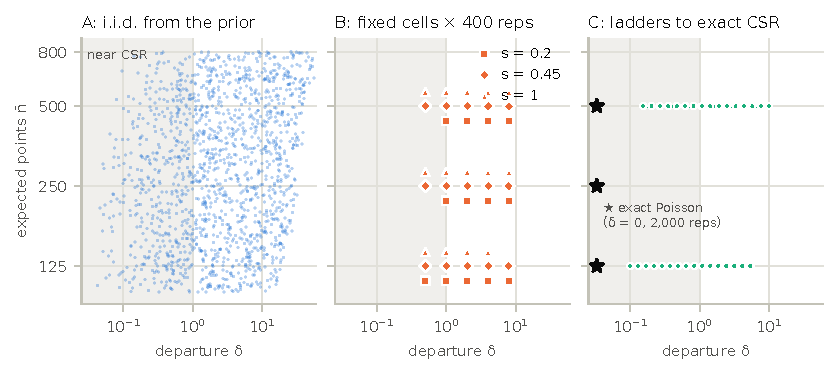
\includegraphics[width=\linewidth]{figs/gen_testsets.pdf}
\caption{Where the three test sets sit in the $(\delta,\nbar)$ plane, for Thomas (closed-form $\dtil$). A fills the plane as $\pi$ does, with 27--40\% of its mass left of $\delta=1$. B places replicated cells on a grid; marker shape marks the scale level, and offsets are for legibility. C runs dense ladders at two $\nbar$ down to $\dtil=0.1$, with exact Poisson anchors at $\delta=0$ (stars).}
\label{fig:testsets}
\end{figure}

% ============================================================================
\section{Validation protocol}\label{sec:valid}

\textbf{Principles.} All five are fixed now, before any data exist.
\begin{enumerate}
  \item[(i)] \emph{Invisibility.} A sampler error is acceptable if it is below a tenth of the null s.d.\ of the relevant summary at the cell's $\nbar$.
  \item[(ii)] \emph{Detectability.} Every check is also a hypothesis test at our replicate count.
  \item[(iii)] \emph{Pre-registration.} The criteria below are fixed now.
  \item[(iv)] \emph{Multiplicity.} Holm correction within each family's battery, at family-wise $\alpha=0.01$.
  \item[(v)] \emph{Blocking.} A failed check blocks the next work package. Reruns are logged and reported, never silent.
\end{enumerate}

\begin{table}[ht]
\centering\small
\begin{tabularx}{\linewidth}{@{}l l L L@{}}
\toprule
Check & Families & What is compared & Pass criterion\\
\midrule
V0 counts & all & mean $n/\nbar$ per B/C cell and over A & $|\text{ratio}-1|\le\max(3\,\text{s.e.},1\%)$\\
V1 $K$ & Poisson, Thomas, nested, Mat\'ern II, LGCP & per B cell: mean $\hat K$ (Ripley isotropic, \emph{true} $\lambda^2$) vs.\ closed form on $\R$ & studentised sup vs.\ its 99\% point (Gaussian bootstrap with the replicate covariance): failing cells at most the 99\% quantile of $\text{Bin}(\#\text{cells},0.01)$, none beyond the 99.99\% point; and $|\bar K-K|\le0.1\,s_0^K$ everywhere\\
V2 dispersion & Poisson, Thomas, nested, LGCP & $\operatorname{Var}(n)/\nbar$ vs.\ $1+\nbar\iint_{W\times W}(g-1)$ (via the set covariance of $W$) & within 3 s.e.\\
V3 hard core & Mat\'ern II; Strauss at $\gamma=0$ & minimum inter-point distance in every pattern & $\ge R$ always (deterministic)\\
V4 edges & Mat\'ern II, Strauss, Thomas, nested & intensity in the band within $\max(R,2\sigma)$ of $\partial W$ vs.\ interior; Strauss also $2R$ vs.\ $4R$ expansion ($n$, $s_R$, $\hat L$) & $|\text{ratio}-1|\le\max(3\,\text{s.e.},1\%)$; no Holm rejection\\
V5 CFTP vs.\ MH & Strauss & 6 settings spanning $F$ including its hardest corner, 1{,}000 draws per sampler: $n$ (mean, var), $s_R$, $\hat L$, $\hat G$, $\hat F$ & no Holm rejection; standardised differences $<0.1$ null s.d.\\
V6 limits & Strauss, Thomas, LGCP & 2{,}000 patterns each at $\nbar=250$ with Strauss $\gamma=1$, Thomas $\mu=10^{-3}$, LGCP $\sigma^2=10^{-3}$, against Poisson: counts and the law of $S$ & dispersion $1\pm3$ s.e.; KS $p>0.01$\\
V7 LGCP numerics & LGCP & every draw: minimum eigenvalue; recorded $M$ against the table; sample covariance of $10^4$ fields at 5 lags & $\ge-10^{-10}\max$; $M$ passes; within 3 s.e.\ of $C$\\
V8 RNG & all & duplicate seeds; correlation of $16\times16$ count maps between equal-index cases of different families; 1\% of cases regenerated & none; within 3 s.e.\ of 0; bit-identical\\
V9 null tables & -- & $c_{0.95}(n)$ from 2{,}000 binomial replicates per $n$ & Monte Carlo s.e.\ $\le0.05$\\
\bottomrule
\end{tabularx}
\caption{Pre-registered checks. V1--V7 first run on dedicated validation batches (WP3), before any bulk generation. V0, V1 and V8 run again on the real data (WP4).}
\label{tab:valid}
\end{table}

\textbf{Review gates.} At each gate you look at output before the next stage starts.
\begin{itemize}
  \item \textbf{D1} (about 21 Sep), after the pilots: $F$, the Strauss lookup residuals, the LGCP resolution table, prior coverage, and the B/C cell list. These are frozen into \code{configs/generation/dv3.yaml} and \code{dv3_cells.csv}. Nothing is generated at scale before you approve them.
  \item \textbf{D2} (about 23 Sep), after the validation batches: V1--V7 all pass.
  \item \textbf{D3} (about 25 Sep), after bulk generation: V0, V1 on the B cells, and V8.
  \item \textbf{D4} (about 30 Sep), after the first training round on A, before any B/C analysis: sanity checks. Skill should be near 0 at $\dhat\le0.5$. An $n$-only baseline should reach chance accuracy in classification.
\end{itemize}

% ============================================================================
\section{How the generation runs}\label{sec:compute}

\textbf{Code layout.} A new package, \code{src/cloudforger/generation/}, reusing the existing samplers where they are correct.
\begin{itemize}
  \item \code{prior.py} reads \code{configs/generation/dv3.yaml} and draws, constrains and inverts.
  \item \code{design.py} solves the B cells and C levels and writes \code{dv3_cells.csv}, which is committed.
  \item \code{seeding.py} builds spawn keys and R seeds.
  \item \code{samplers/} holds \code{poisson}, \code{neyman_scott} (reused), \code{matern2} (fixed), \code{lgcp_ce} (new), \code{strauss_r} (the R bridge) and \code{strauss_mh} (the fallback).
  \item \code{store.py} writes shards and manifests; \code{validate.py} implements V0--V9.
\end{itemize}
Command-line entry points go in \code{scripts/generation/}: \code{plan}, \code{run_shard}, \code{merge}, \code{validate}, \code{regen_case}, plus \code{strauss_cftp.R}. SLURM wrappers go in \code{slurm/gen_*.sh}, and this time \code{slurm/} is committed (audit \S5.12).

\textbf{The plan.} One short job enumerates every case into \code{plan.csv}, about 204{,}000 rows. Each row has the case id, set, family, index, cell or level, and spawn key, plus, for training and A, the drawn $\theta$. The plan is deterministic given \code{dv3.yaml} and \code{dv3_cells.csv}, and its checksum is recorded. Steps 1--3 of Fig.~\ref{fig:pipeline} happen here.

\textbf{Random numbers.} Every case gets its own streams:
{\footnotesize
\begin{verbatim}
ROOT = <128-bit integer, drawn once with secrets.randbits(128), stored in dv3.yaml>
key  = (3, set_id, family_id, index, role)        # 3 = dataset version DV3
rng  = numpy.random.Generator(PCG64DXSM(SeedSequence(ROOT, spawn_key=key)))

set_id    : train 0, A 1, B 2, C 3, pilot 8, validation 9
family_id : poisson 0, thomas 1, nested 2, matern2 3, strauss 4, lgcp 5
role      : 0 = parameters, 1 = pattern
index     : training/A running index; B 10000*cell + rep; C 1000000*ladder + 10000*level + rep
R seed    : SeedSequence(ROOT, spawn_key=key).generate_state(1)[0] mod (2^31 - 1) + 1,
            uniqueness checked over all Strauss cases; RNGkind pinned
\end{verbatim}
}
\emph{Why this layout.}
\begin{itemize}
  \item Any case can be regenerated alone.
  \item Parameters and patterns use different streams, so upgrading a sampler never changes $\theta$.
  \item Families and sets never share a stream. DV1's twins (audit \S5.14) and its reuse of the design stream for cloud~0 are impossible by construction.
  \item \code{SeedSequence} hashes the key, so neighbouring keys give statistically independent streams. \code{PCG64DXSM} is numpy's generator for massively parallel use. A counter-based Philox generator \citep{Salmon2011} would serve equally well.
\end{itemize}

\textbf{Shards and jobs.} A shard is about 500 cases of one (set, family), sorted by $\nbar$ so that shards cost about the same.
\begin{itemize}
  \item \emph{Generation.} About 410 SLURM array tasks, each on 1 CPU with 4\,GB (8\,GB for LGCP), under an hour each. A task reads its rows of \code{plan.csv}, simulates, and writes one shard file.
  \item \emph{The Strauss route.} A Strauss shard writes a CSV of (case id, $\beta$, $\gamma$, $R$, R seed). It calls \code{Rscript strauss_cftp.R} once, which loops over cases with \code{set.seed} and \code{rStrauss}, and reads the points back. R starts once per shard (about 1\,s), and the R library lives in \texttt{\$HOME}, safe from the scratch purge.
  \item \emph{Resumability.} Tasks are idempotent: a shard that exists with a valid checksum is skipped. Failures rerun with the same seeds. \code{merge} refuses to write a set with any case missing, so no case is ever silently dropped.
  \item \emph{Diagrams.} These use the existing shard$\to$merge pipeline (\code{diagrams_shard.py}). Shards are sized by $\sum n^{3.1}$, with 24\,GB per task (48\,GB for LGCP, because of its count tail).
\end{itemize}

\textbf{Storage.} Each (set, family) lives in \code{data/dv3/<set>/<family>/}.
\begin{itemize}
  \item \code{points.npz} holds all coordinates as one float64 array plus int64 offsets.
  \item \code{manifest.csv} has one row per case (Table~\ref{tab:manifest}).
  \item \code{clouds.pkl} is a compatibility copy in the current record format, so the existing featurisation runs unchanged.
\end{itemize}
Patterns are the canonical record. Seeds regenerate cases but are not a substitute for storage: numpy guarantees identical streams only on the same build and machine. All patterns together take about 2\,GB. Every derived cache (diagrams, $L$/$F$/$G$) records \code{DV3} and the SHA-256 of \code{points.npz}, and loaders refuse a mismatch; this fixes the stale-cache hazard of audit \S5.10. A dataset card records the \code{dv3.yaml} hash, the git commit (a clean tree is required), and the numpy, scipy, gudhi, R and spatstat.random versions.

\begin{table}[ht]
\centering\small
\begin{tabularx}{\linewidth}{@{}l L@{}}
\toprule
Group & Columns\\
\midrule
identity & \code{case_id}, \code{dv}, \code{set}, \code{family}, \code{index}, \code{cell_id}/\code{level_id}, \code{rep}, \code{spawn_key}, \code{r_seed}, \code{split}\\
design & \code{nbar} and the family's coordinates (\code{mu}, \code{s}, \code{mu1}, \code{mu2}, \code{s2}, \code{rho}, \code{tau}, \code{gamma}, \code{sigma2}, \code{sp})\\
model & \code{kappa}, \code{sigma}, \code{sigma1}, \code{lam_p}, \code{R}, \code{beta}, \code{mu_log}, \code{s_abs}\\
regime & \code{delta_tilde}, \code{tau_K}, \code{n} (realised)\\
sampler & \code{sampler} (\code{exact}/\code{cftp}/\code{mh}), \code{buffer}, \code{n_parents}, \code{grid_M}, \code{pad_P}, \code{min_eig}, \code{cftp_start}, \code{mh_steps}, \code{burnin}, \code{wall_s}, \code{sha1}\\
\bottomrule
\end{tabularx}
\caption{Manifest columns: one row per pattern.}
\label{tab:manifest}
\end{table}

\textbf{Regenerating one case.} \code{regen_case --case <id>} does four things.
\begin{enumerate}
  \item Read the case's manifest row.
  \item Rebuild the spawn key.
  \item For training and A, redraw $\theta$ and compare it with the stored value.
  \item Rerun the sampler and compare the result with the stored pattern: bit-for-bit in the same environment, distributionally otherwise.
\end{enumerate}
App.~\ref{app:worked} traces one case from id to file.

\begin{figure}[ht]
\centering
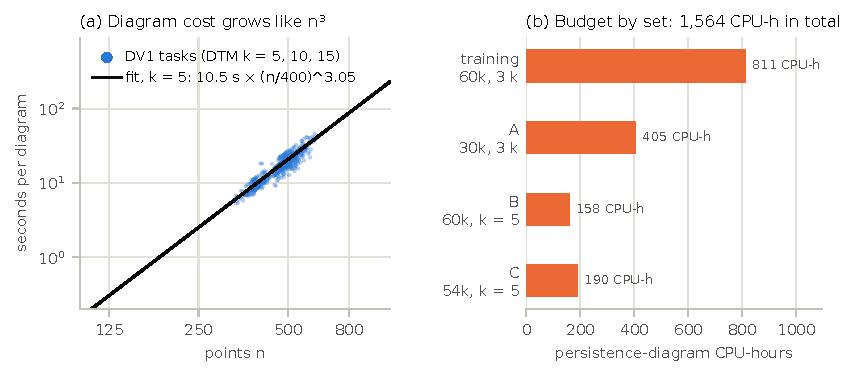
\includegraphics[width=\linewidth]{figs/gen_cost.pdf}
\caption{(a) Why the largest $\nbar$ sets the price of the study. Seconds per DTM persistence diagram against points, for the DV1 diagram jobs (1{,}262 tasks, SLURM accounting). The fitted law is $10.5\,\text{s}\times(n/400)^{3.05}$ for $k=5$, similar for $k=10,15$. (b) Diagram budget by set: all three $k$ for training and A, $k=5$ only for B and C (decision 11).}
\label{fig:cost}
\end{figure}

\textbf{Compute budget.}
\begin{itemize}
  \item \emph{Simulation} is cheap except possibly Strauss. Poisson, Neyman--Scott and Mat\'ern~II take well under 0.1\,s per pattern, and LGCP 0.1--0.5\,s. Strauss by CFTP is unknown \openflag. The MH fallback costs 0.3--6\,s (DV1: 0.27--0.6\,s at 40 sweeps \measured, times 10 for burn-in by coupling). That is at most 100 CPU-h in all.
  \item \emph{Persistence diagrams} dominate (Fig.~\ref{fig:cost}): about 30\,s per cloud at $n=400$ for three DTM filtrations, but about 4\,min at $n=800$. The totals are 811 (training), 405 (A), 158 (B) and 190 (C) CPU-h, i.e.\ 1{,}564 CPU-h. This assumes a 20\% allowance for the realised-count tail. At the roughly 600 concurrent slots the DV1 jobs used, that is 1--2 days of wall time including queueing.
  \item \emph{Summary curves} ($L,F,G$) take about 20 CPU-h.
  \item \emph{Training and evaluation} take about 50--80 GPU-h. The audit's to-run list is about 21 GPU-h at 7{,}000 clouds per family, scaled by 1.5 for the 10{,}000-cloud pools and increased for restarts and evaluation.
\end{itemize}

% ============================================================================
\section{Threats to validity, and how the paper should describe the design}\label{sec:threats}

\begin{enumerate}
  \item \emph{Prior dependence of A.} Log-uniform in dimensionless coordinates is a choice. Mitigation: A is reweighted to alternative priors on the same support; report the headline's sensitivity.
  \item \emph{Shrinkage in B and C.} A $\pi$-trained estimator is biased towards the prior mean, most near CSR and near support edges. Mitigation: the interior rule, and skill reported per cell.
  \item \emph{What $\delta$ means.} $\delta$ is the $L$ test's difficulty on this window, estimator and radius range. It compares families only under this pipeline, and it is blind below $r=0.01$ (\S\ref{sec:delta}). Being second order, it can also miss structure entirely: a non-Poisson process can have the $K$ of CSR \citep{BaddeleySilverman1984}.
  \item \emph{Simulation approximations.} Neyman--Scott buffers ($\le10^{-5}$ of points), Strauss on $W\oplus2R$ (V4), the LGCP grid (V1 against the continuous $K$), and the Strauss prior truncated to $F$, with MH only where declared. All are bounded, recorded per case and reported.
  \item \emph{Shape priors that depend on $\nbar$.} Truncation at small $\nbar$ (nested: 61\% of shapes rejected at $\nbar=125$). Disclosed; nested claims are made at $\nbar\ge250$ only.
  \item \emph{Model scope.} Stationary, isotropic models on one window size only. Nothing here speaks to inhomogeneous data.
  \item \emph{Training non-determinism} (audit \S5.6). Analyses use paired per-cloud differences with a seed-level bootstrap.
  \item \emph{Multiplicity} across cells, families and statistics. Pre-register the primary cells and metrics, and apply Holm correction to the rest.
\end{enumerate}

\begin{keybox}
\textbf{Suggested wording for the paper.} ``All networks are trained on simulations from a prior $\pi$ over each model's parameters (Table~X). We report test performance in two ways. Test set A is an independent sample from $\pi$. Its average loss estimates each network's integrated risk under $\pi$, the quantity a Bayesian procedure minimises, and is the basis for comparison with methods that use the same prior. Test sets B and C instead fix the parameters. B uses a grid of values that spans sample size and distance from complete spatial randomness. C uses one-parameter paths that end at complete spatial randomness. Every parameter value in B and C lies in the interior of the support of $\pi$, so these are not out-of-distribution tests. They measure the frequentist behaviour (bias, error, detection power) of estimators trained to be optimal on average under $\pi$. Near the limit of identifiability such estimators shrink towards the prior, and we report this explicitly as skill relative to the prior mean.''
\end{keybox}

% ============================================================================
\section{Implementation plan}\label{sec:plan}

\begin{table}[ht]
\centering\small
\begin{tabularx}{\linewidth}{@{}l L l l L@{}}
\toprule
WP & What & Needs & Compute & Output; gate\\
\midrule
0 & Tag DV1/DV2 (\code{dv1-final}); commit \code{slurm/}; move \code{cloud-env} off scratch; run \code{install_spatstat.sh}; draw ROOT & -- & none & versions file, tags\\
1 & Generation library, including the Mat\'ern~II fix and circulant LGCP; unit tests for limits ($\gamma=1$, $\mu\to0$, round-trip inversions, minimum distances) & 0 & none & code\\
2 & Pilots. (a) null tables: 2{,}000 binomial replicates at 20 values of $n$; (b) CFTP timing probe (\code{strauss_cftp_probe.sh}); (c) Strauss lookup $h$ plus mean-curve tables over $F$; (d) LGCP resolution table; (e) final coverage and B/C cell solve & 1 & $\le60$ + $\le50$ + 2 CPU-h & \code{dv3.yaml}, \code{dv3_cells.csv}; \textbf{D1}\\
3 & Validation batches (set 9), V1--V7 & 2 & $\approx40$ CPU-h & report; \textbf{D2}\\
4 & Plan; generate every shard; merge; V0, V1 on B, V8 & 3 & $\le100$ + 10 CPU-h & \code{data/dv3/}; \textbf{D3}\\
5 & Diagrams (training and A: 3 DTM $k$ + Rips; B and C: $k=5$ + Rips) and $L$/$F$/$G$ caches, stamped with the version & 4 & $\approx1{,}600$ CPU-h & features\\
6 & Training side: loaders honour \code{split} and the DV3 stamp; save per-cloud predictions; 6-class bundle; classification paths for Betti curves and landscapes; B/C evaluation harness & 1 & none & code\\
7 & Train the matrix and headline configurations (10 seeds); evaluate on A, B, C & 5, 6 & 50--80 GPU-h & results; \textbf{D4} after the first round on A\\
8 & Analysis, figures, writing & 7 & small & paper\\
\bottomrule
\end{tabularx}
\caption{Work packages. WP6 runs in parallel with WP2--WP5. Inside WP4 every set and family runs in parallel. WP5 starts on each set as soon as it is merged, training first.}
\label{tab:wp}
\end{table}

\begin{figure}[ht]
\centering
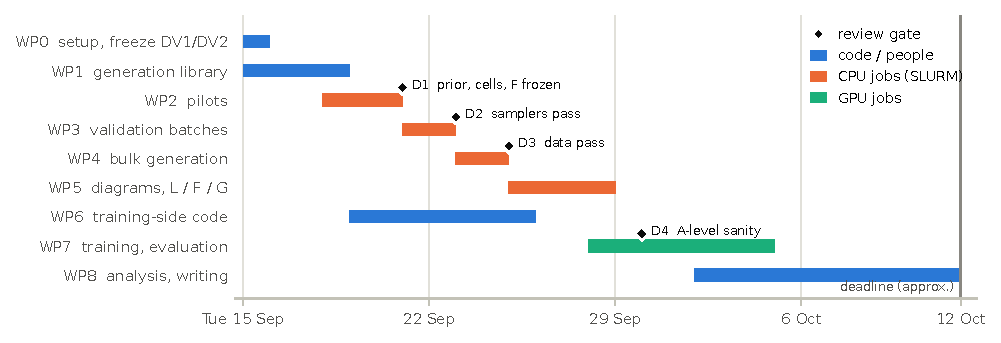
\includegraphics[width=\linewidth]{figs/gen_gantt.pdf}
\caption{Schedule, assuming a deadline of 12 October. The critical path is WP1$\to$2$\to$3$\to$4$\to$5$\to$7$\to$8, about 20 days, leaving roughly a week for analysis and writing. The biggest schedule risk is WP2(b): if CFTP is infeasible over much of the Strauss prior, the pre-declared MH fallback takes over there, and V5 compares the two where both run.}
\label{fig:gantt}
\end{figure}

The review gates D1--D4 and what you look at in each are listed in \S\ref{sec:valid}.

\textbf{What has already been prepared (this session).} All of it is in \code{docs/theory/scripts/}. The install and probe scripts have \emph{not} been run. \code{design_preview.py} was run (closed forms and saved tables only) to produce this document's \measured{} design numbers.
\begin{itemize}
  \item \code{install_spatstat.sh}, \code{strauss_cftp_probe.R} and \code{strauss_cftp_probe.sh}, for WP0 and WP2(b);
  \item the probe grid, \code{out/strauss_probe_grid.csv} (72 cells, $\beta$ from the DV1 lookup);
  \item \code{design_preview.py}, whose output is WP2(e) in preview form.
\end{itemize}

% ============================================================================
\section{Open items}\label{sec:open}
\begin{enumerate}
  \item The CFTP-feasible region $F$, hence the Strauss $\tau$ upper bound for each $\gamma$ (WP2b; D1).
  \item The Strauss B cells, C ladder range and prior coverage, which need the pilot mean curves (WP2c).
  \item Whether \code{spatstat.random} compiles in the R~4.5.1 container (WP0). If not, the fallback is MH with coupling-based burn-in, used everywhere and validated by V4 and V6. V5 would then have no CFTP reference.
  \item The LGCP grid table and the padding needed for the exponential covariance. $P=2$ is expected for $s\le0.15$, but this is unverified.
  \item Primary $\delta$ for inhibitory families: $\delta_L$ is blind below $r=0.01$; decide at D1 whether B/C analyses of Mat\'ern~II and Strauss use $\delta_G$.
  \item Whether 10{,}000 training patterns per family suffice for the wider prior. Check the learning curves at D4.
  \item The exact deadline date.
  \item \code{cloud-env} is on purgeable scratch; relocate it in WP0.
  \item DV1's Neyman--Scott counts sit 0.4\% low ($z\approx-2$, with no known mechanism). V0 on A resolves this at 0.24\% precision.
  \item Memory for the LGCP count tail in diagram jobs. If 48\,GB fails, those shards need a high-memory queue.
\end{enumerate}

% ============================================================================
\appendix
\section{Short derivations}\label{app:deriv}

\subsection{Why $\delta$ grows like $\sqrt{\nbar}$}\label{app:counting}
Take CSR with $n$ points in the unit square and small $r$, ignoring edges. The number of pairs within distance $r$ is close to Poisson with mean $n^2\pi r^2/2$. Since $\hat K=2P/n^2$, we get $\operatorname{sd}\hat K(r)\approx\sqrt{2\pi}\,r/n$. A process with $K=\pi r^2+e(r)$ shifts $\E\hat K$ by $e(r)$ to first order, so it stands $z(r)=\nbar\,e(r)/(\sqrt{2\pi}\,r)$ null standard deviations from CSR. Studentising $\hat L-r$, a smooth monotone transform of $\hat K$, gives the same $z$ to first order.

For Thomas, $e(r)=(\mu/\nbar)(1-e^{-r^2/4\sigma^2})$. With $x=r/2\sigma$, the factor $(1-e^{-x^2})/x$ peaks at $0.638$ at $x\approx1.12$. So $z_{\max}=0.638\,\mu/(2\sqrt{2\pi}\,\sigma)=0.127\,\mu/\sigma=0.127\,\mu\sqrt{\nbar}/s$, and with $c_{0.95}\approx3.2$, $\delta\approx0.04\,\mu\sqrt{\nbar}/s$. This holds provided the peak radius $2.24\,\sigma$ lies in $\R$. For Mat\'ern~II, $e(r)=-\pi r^2$ for $r<R$, so $z(R)\approx1.25\,\tau\sqrt{\nbar}$. The deficit is visible to $\delta_L$ only once $R\ge0.01$.

\subsection{Monte Carlo errors}\label{app:mc}
Let a cell have $m$ replicate errors $e_i$ with mean $b$, s.d.\ $\sigma_e$ and kurtosis $\kappa_4$ ($m=400$ in B, 300 in C).
\begin{itemize}
  \item Bias: $\operatorname{se}(\bar e)=\sigma_e/\sqrt{m}$.
  \item MSE (at $b=0$): $\operatorname{Var}(e^2)=(\kappa_4-1)\sigma_e^4$. So the relative s.e.\ of the MSE is $\sqrt{(\kappa_4-1)/m}$, and by the delta method that of the RMSE is half of it.
  \item Paired difference of two methods with equal error variance and correlation $\rho$ (Gaussian): $\operatorname{Var}(e_A^2-e_B^2)=4\sigma_e^4(1-\rho^2)$. So the relative s.e.\ of the MSE difference is $2\sqrt{1-\rho^2}/\sqrt{m}$.
  \item A proportion (recall, power): s.e.\ $\le\sqrt{0.25/m}$.
  \item Achieved size from $N_0=2{,}000$ Poisson scores: $\sqrt{0.05\cdot0.95/N_0}=0.49$ points.
\end{itemize}

\subsection{Mat\'ern~II inversion}\label{app:m2}
From $\pi R^2\lambda=1-e^{-\lambda_p\pi R^2}$ we get $\lambda_p=-\ln(1-\pi R^2\lambda)/(\pi R^2)$. With $\lambda=\nbar$ and $R=\tau/\sqrt{\nbar}$, $\pi R^2\lambda=\pi\tau^2$, so $\lambda_p=\nbar\,[-\ln(1-\pi\tau^2)]/(\pi\tau^2)$. At $\tau=0.55$ that is $3.16\,\nbar$.

\subsection{Strauss scale invariance}\label{app:scale}
Let $X$ have density $f(x)\propto\beta^{n(x)}\gamma^{s_R(x)}$ on $A$ with respect to the unit-rate Poisson process. The map $x\mapsto ax$ sends that Poisson process to one of rate $a^{-2}$ on $aA$. Re-expressing the density against the unit-rate process on $aA$ multiplies it by $a^{-2n}$ up to a constant. Also $s_R(x)=s_{aR}(ax)$. Hence $aX$ is Strauss$(\beta/a^2,\gamma,aR)$ on $aA$: intensity scales as $a^{-2}$ and range as $a$, so $\lambda R^2$ depends only on $(\beta R^2,\gamma)$ for the stationary process. The finite window breaks this only through edge effects, which the DV1 fit shows to be negligible (\S\ref{sec:strauss}).

\subsection{Neyman--Scott buffer error}\label{app:buffer}
A point at distance $u$ from one side of $W$ has its parent beyond a buffer of width $b$ on that side iff its offset along that axis exceeds $u+b$. Summing over the four sides (an upper bound, since corners are counted twice), the expected fraction of missing points is at most $4\int_0^\infty P(\sigma Z>u+b)\dd u=4\sigma\,\E(Z-b/\sigma)^+$. Here $\E(Z-a)^+=\varphi(a)-a(1-\Phi(a))$, which equals $2.4\times10^{-5}$ at $a=3.719$. So the fraction is at most $10^{-4}\sigma$, i.e.\ at most $10^{-5}$ for $\sigma\le0.1$. The nested process pays this once per level.

\section{Worked example: one Thomas training case, from id to file}\label{app:worked}
The parameter values below are illustrative; the arithmetic is exact.
\begin{enumerate}
  \item \emph{Identify.} \code{dv3-train-thomas-000417} has spawn keys $(3,0,1,417,0)$ for its parameters and $(3,0,1,417,1)$ for its pattern.
  \item \emph{Draw $\theta$.} The parameter stream gives $u=0.547$, so $\nbar=100\cdot8^{0.547}=312$; then $\mu=4.0$ and $s=0.40$. Constraints: $\sigma=0.40/\sqrt{312}=0.0226\le0.1$ and $\kappa=312/4=78\ge5$, so the draw is accepted.
  \item \emph{Invert.} $\kappa=78.0$, $\mu=4.0$, $\sigma=0.0226$. Also $\tau=1.665\,s=0.666$, and $\dtil=6.1$ \measured. The rule of thumb of App.~\ref{app:counting} gives $0.04\cdot4\cdot17.7/0.4=7.1$.
  \item \emph{Simulate} with the pattern stream. The buffer is $b=3.719\,\sigma=0.0842$, so parents fall on $[-0.084,1.084]^2$ (area $1.365$). Draw $N_p\sim\Pois(106.5)$ parents; each has $\Pois(4)$ children with $N(0,0.0226^2I)$ offsets; keep the children in $W$. The expected count is 312.
  \item \emph{Store.} Append the points to the (train, thomas) shard. The manifest row records $\nbar,\mu,s$; $\kappa,\sigma$; $\dtil,\tau$; the realised $n$; \code{sampler=exact}, the buffer, $N_p$, wall time, the hash; and its \code{split}.
  \item \emph{Check.} Training cases are not tested one by one: V0 and V1 run on A and the B/C cells. This case enters V8's 1\% regeneration sample if it is drawn, and anyone can reproduce it with \code{regen_case --case dv3-train-thomas-000417}.
\end{enumerate}

\bibliographystyle{plainnat}
\bibliography{generation}

\end{document}
